%%16:58:54 6/5/2015 -VieTeX creates F:\1HIEP HOC\LUANVAN\baocao\daydu.tex
\documentclass[notheorems,envcountsect,hyperref=unicode]{beamer}
\usetheme{Darmstadt}
\usefonttheme[onlylarge]{serif}
\setbeamerfont*{frametitle}{size=\normalsize,series=\bfseries}
% Standard packages
\usepackage{amsmath,amssymb,amsxtra,latexsym, amscd,amsfonts,amsthm}
\usepackage{longtable}
\usepackage[utf8]{vietnam}
\usepackage[english]{babel}
\usepackage{verbatim}
\usepackage{indentfirst}
\usepackage{ragged2e}
\usepackage{mathrsfs}
\usepackage{commath}
\usepackage{cases}
\justifying
% Setup TikZ
\usepackage{tikz}
\usetikzlibrary{arrows}
\tikzstyle{block}=[draw opacity=0.7,line width=1.4cm]
\newtheorem{nx}{Nhận xét}[section]
\newtheorem{dl}{Định lý}[section]
\newtheorem{bd}{Bổ đề} [section]
\newtheorem{dn}{Định nghĩa}[section]
\newtheorem{vd}{Ví dụ} [section]
\newtheorem{hq}{Hệ quả}[section]
\newtheorem{cm}{Chứng minh}
\newtheorem{bt}{Bài tập}
\newcommand{\R}{\mathbb R} 
\newcommand{\N}{\mathbb N} 
\newcommand{\E}{\mathbb E}
\newcommand{\Q}{\mathbb Q}
\newcommand{\Om}{\Omega}
\newcommand{\BOm}{\partial\Omega}

\def\A{\mathcal{A}}
\def\C{\mathbb{C}}
\def\R{\mathbb{R}}
\def\Q{\mathbb{Q}}
\def\Z{\mathbb{Z}}
\def\N{\mathbb{N}}
\def\L{\mathcal{L}}
\def\ln{\ell_p^n}
\def\l1{\ell_1}
\def\lp{\ell_p}
\def\lq{\ell_q}
\def\lo{\ell_{\infty}}
\def\Lp{\mathbf{L_p}}
\def\Lpp{\mathit{L_p}}
\def\Lqq{\mathit{L_q}}
\def\Lo{\mathbf{L_{\infty}}}
\def\Loo{\mathit{L_{\infty}}}
\def\m{\mu}
\def\s{\sigma}
\def\sgn{\text{sign}}
\def\disint{\displaystyle\int}
\def\dissum{\displaystyle\sum}
\def\van{triệt tiêu bên ngoài một tập có độ đo hữu hạn }
\def\hol{bất đẳng thức Hölder }
\def\hkn{hầu khắp nơi}
\def\es{\text{ess sup}}
\def\kgdd{(X,\A,\mu)}

%%%%%%%%%


\def\nga{\widetilde}
\def\ex{\begin{example}
	}
	\def\eex{\end{example}}
\def\thr{\begin{satz}}
	\def\ethr{\end{satz}}
\def\pro{\begin{Proposition}}
	\def\epro{\end{Proposition}}
\def\coro{\begin{Korollar}}
	\def\ecoro{\end{Korollar}}
\def\df{\begin{definitionsatz}}
	\def\edf{\end{definitionsatz}}
\def\lm{\begin{axiom}}
	\def\elm{\end{axiom}}
\def\pf{\begin{proof}}
	\def\epf{\end{proof}}
\def\problem{\begin{problem}}
	\def\eproblem{\end{problem}}
\def\dlim{\displaystyle\lim}
\def\csd{\underset}
\def\hoi{\wedge}
\def\it{\begin{itemize}}
	\def\hit{\end{itemize}}
\def\rem{\begin{remark}}
	\def\erem{\end{remark}}
\def\ss{\parallel}
\def\cla{\begin{claim}}
	\def\ecla{\end{claim}}
\def\it{\begin{itemize}}
	\def\hit{\end{itemize}}





\begin{document}
	\begin{frame}{\MakeUppercase{\textsc\bf\small{\centerline{Bộ Giáo dục và Đào tạo} \newline\centerline{Trường Đại Học Quy Nhơn}}}}
	\vspace*{0.2cm}
	
    \centerline{\MakeUppercase{\textsc{\bf\small{NGUYỄN NHẬT NAM}}}}
    \vspace*{0.8cm}
	
%	\centerline{\large\alert{\MakeUppercase{\textsc{\bf{ MỘT SỐ PHƯƠNG PHÁP PHÂN TÍCH DỮ LIỆU VÀ ỨNG DỤNG}}}}}
	\centerline{\large\alert{\MakeUppercase{\textsc{\bf{ MỘT SỐ PHƯƠNG PHÁP}}}}}
	\centerline{\large\alert{\MakeUppercase{\textsc{\bf{ PHÂN TÍCH DỮ LIỆU VÀ ỨNG DỤNG}}}}}


	\vspace*{0.9cm}
		\centerline{\bf{KHÓA LUẬN TỐT NGHIỆP ĐẠI HỌC}}
		\centerline{\bf{Ngành: TOÁN ỨNG DỤNG }}
	\vspace*{0.6cm}
	\centerline{Người hướng dẫn} \MakeUppercase{\centerline{\textsc\bf{ TS.LÂM THỊ THANH TÂM}}}
	\vspace*{0.3cm}	
	\centerline{Bình Định, 2023}
\end{frame}
\begin{frame}
\renewcommand{\baselinestretch}{1.5}
	\frametitle{\MakeUppercase{\textsc\bf\large{Mở đầu}}}
	
    
Nội dung khóa luận được trình bày trong 4 chương:
	\begin{itemize}
		
		\item\textbf{Chương 1. Một số kiến thức chuẩn bị}
		
		\item\textbf{Chương 2. Phân tích giá trị kì dị (SVD)}
		
		\item\textbf{Chương 3. Phân tích thành phần chính (PCA)}
		
		\item\textbf{Chương 4. Một số ứng dụng của SVD và PCA}
		
	\end{itemize}
\end{frame}
%\begin{frame}{Chương 2. Phân tích giá trị kì dị (SVD)}
%\begin{block}{\textnormal{Định nghĩa}}
%Cho $1\leq p<\infty$. \textbf{Không gian dãy Lebesgue}, ký hiệu là $\lp$, là tập hợp các dãy số thực $\mathbf{x}=\lbrace x_n\rbrace_{n\in\N}$ sao cho $\dissum_{n=1}^{\infty} \vert x_n\vert^p<\infty$, và một ánh xạ trên không gian này được xác định bởi
%\begin{align*}
%\Vert \mathbf{x}\Vert_{\lp}=( \sum_{n=1}^{\infty} \vert x_n\vert^p)^{\frac{1}{p}},\quad \mathbf{x}=\lbrace x_n\rbrace_{n\in\N}\in\lp.
%\end{align*}
%\end{block}

%\begin{block}{\textnormal{Định nghĩa}}
%\textbf{Không gian dãy bị chặn}, ký hiệu là $\lo$, là tập hợp các dãy số thực $\lbrace x_n\rbrace_{n\in\N}$ bị chặn cùng với ánh xạ được cho bởi
%\begin{align*}
%\Vert \mathbf{x}\Vert_{\lo}=\sup_{n\in\N} \vert x_n\vert, \quad \mathbf{x}=\lbrace x_n\rbrace_{n\in\N} \in\lo.
%\end{align*}
%\end{block}
%\end{frame}

\begin{frame}{Chương 2. Phân tích giá trị kì dị (SVD)}
\begin{itemize}
\item \textbf{Định lí về sự tồn tại của SVD }
\item \textbf{Thuật toán SVD}
\end{itemize}
\end{frame}
\begin{frame}{Chương 2. Phân tích giá trị kì dị (SVD)}
	\begin{block}{\textnormal{Định lý}} Cho $\mathbf{A}$ là một ma trận có cấp $m \times n$. Khi đó, mọi giá trị riêng của ma trận $\mathbf{A}^{T} \mathbf{A}$ đều không âm.
	\end{block}
	
\end{frame}

\begin{frame}{Chương 2. Phân tích giá trị kì dị (SVD)}
\begin{block}{\textnormal{Định lý}}
Mọi ma trận $\mathbf{A}$ cỡ $m \times n$ bất kì đều có phân tích SVD có dạng

\begin{equation*}
	\mathbf{A}=\mathbf{U D V}^{T}.
\end{equation*}
\end{block}

\end{frame}

\begin{frame}{Chương 2. Phân tích giá trị kì dị (SVD)}
\begin{block}{\textnormal{Định lý}}
Cho $\mathbf{A}$ là ma trận cỡ $m \times n$ bất kì. Khi đó
\begin{equation*} \label{eq_4}
	\mathbf{A}=\mathbf{U D V}^{T}=\sigma_{1} \mathbf{u}_{1} \mathbf{v}_{1}^{T}+\sigma_{2} \mathbf{u}_{2} \mathbf{v}_{2}^{T}+\cdots+\sigma_{r} \mathbf{u}_{r} \mathbf{v}_{r}^{T}.
\end{equation*}
trong đó $\sigma_{i}$ là các giá trị kì dị dương của ma trận $\mathbf{A}, \mathbf{u}_{i}$ là các vector kì dị trái và $\mathbf{v}_{i}$ là các vector kì dị phải của ma trận $\mathbf{A}$.
\end{block}
\end{frame}

%\begin{frame}{Chương 2. Phân tích giá trị kì dị (SVD)}
%\begin{block}{\textnormal{Định lý}}
%	Cho $1\leq p< \infty$ và $q$ liên hợp với $p$. Khi đó, đối ngẫu của không gian $\lp$ là $\lq$.
%\end{block}
%
%Xét quy tắc $T$ được định nghĩa bởi 
%$$T(f)=\lbrace f(e_k)\rbrace_{k\in \N}, \forall f\in (\lp)^*$$
%trong đó $e_k=(0,0,\ldots,0,1,0,\ldots),$ với $1$ ở vị trí thứ $k$. Ta chứng minh:
%\begin{itemize}
%\item Ảnh $T$ thuộc $\lq$
%\item $T$ tuyến tính
%\item $T$ song ánh
%\item $T$ liên tục
%\item $T$ bảo toàn chuẩn
%\end{itemize} 
%\end{frame}

\begin{frame}{Chương 2. Phân tích giá trị kì dị (SVD)}
\begin{block}{\textnormal{Thuật toán SVD}}
\begin{itemize}
\item{Bước 1:} Tính ma trận $\mathbf{A}^{T} \mathbf{A}$  và giải phương trình $\operatorname{det}\left(\mathbf{A}^{T} \mathbf{A}-\lambda \mathbf{I}\right)=0$ từ đó suy ra các giá trị kì dị của $\mathbf{A}$ là $\sigma_{i}=\sqrt{\lambda_{i}}, i=\overline{1, n}$ và $\mathbf{D}=\operatorname{diag}\left(\sigma_{1}, \sigma_{2}, \ldots, \sigma_{n}\right)$.
\item{Bước 2:} Với mỗi giá trị riêng $\lambda_{i}$, tìm vector riêng $\mathbf{v}_{i}$. Từ đó tìm được ma trận trực giao $\mathbf{V}$ cấp $n$ chứa các vector kì dị phải của $\mathbf{A}$.
\item{Bước 3:} Tìm ma trận trực giao $\mathbf{U}$ với 
$$
\mathbf{u}_{i}=\frac{1}{\sigma_{i}} \mathbf{A} \mathbf{v}_{i}.
$$
\end{itemize}
\end{block}

%\begin{itemize}
%\item Đặt $M=\left\lbrace \mathbf{q}=(q_1,\ldots,q_n,0,\ldots):q_k\in\Q,1\leq k\leq n \right\rbrace$. Ta chứng tỏ $M$ trù mật trong $\lp$, $1\leq p<\infty$. Tức là 
%$$\forall \mathbf{x}_n\in\lp,\exists \mathbf{q}\in M:\Vert \mathbf{x}_n -\mathbf{q}\Vert_{\lp}<\epsilon.$$
%\item Lấy bất kỳ dãy đếm được $M=\lbrace \mathbf{x}_n\rbrace_{n\in\N}$ trong $\lo$
%Ta sẽ chứng minh tồn tại $\mathbf{y}\in \lo$ sao cho với mọi $\mathbf{x}_n$ trong $M$
%$$\Vert \mathbf{y}-\mathbf{x}_n\Vert_{\lo}>1.$$
%\end{itemize}
\end{frame}

%\begin{frame}{Chương 2. Phân tích giá trị kì dị (SVD)}
%\begin{block}{\textnormal{Định lý}}
%Nếu $0<p<q< \infty$ thì $\lp \varsubsetneq\lq$.
%\end{block}

% Xét dãy $\lbrace x_n\rbrace_n$ được cho bởi công thức $x_n=n^{-\frac{1}{p}},\forall n\in\N$. Khi đó  với $1\leq p<q\leq \infty$
%$$\dissum_{n=1}^{\infty}\vert x_n\vert^{q}=\dissum_{n=1}^{\infty}\dfrac{1}{n^{q/p}}<\infty.$$
%Tuy nhiên chuỗi
%$$\dissum_{n=1}^{\infty}\vert x_n\vert^{p}=\dissum_{n=1}^{\infty}\dfrac{1}{n}$$
%phân kỳ.
%\end{frame}

\begin{frame}
	\frametitle{\MakeUppercase{\textsc\bf\large CHƯƠNG 3. Phân tích thành phần chính}}
	\renewcommand{\baselinestretch}{1.5}
	\begin{itemize}
		\item [3.1] \textbf{Ý Tưởng}
		\item [3.2] \textbf{Phân tích thành phần chính }
		%\pause
%		\item [3.3] \textbf{Mối liên hệ giữa PCA và SVD }
		%\pause
		\item [3.3] \textbf{Tính duy nhất nghiệm của PCA}
		%\pause
		\item [3.4] \textbf{Thuật toán PCA}
	\end{itemize}
\end{frame}
\begin{frame}{3.1 Ý Tưởng }
%Cho $\kgdd$ là một không gian độ đo và $f$ là một hàm đo được. Ta định nghĩa \textbf{cận trên cốt yếu} của $f$, ký hiệu $\Vert f\Vert_{\infty}$, được xác định bởi
%$$\Vert f\Vert_{\infty}=\inf\left\lbrace M>0:\m\left( x\in X:\vert f(x)\vert >M\right)=0\right\rbrace.$$
%với quy ước rằng $\inf(\emptyset)=+\infty$.
Tìm một phép xoay trục toạ độ để được một hệ trục toạ độ mới sao cho trong hệ mới này, thông tin của dữ liệu chủ yếu tập trung ở một vài thành phần. Phần còn lại chứa ít thông tin hơn có thể được lược bỏ.
%\begin{block}{\textnormal{Định nghĩa}}
% \textbf{Tập hợp các hàm bị chặn hầu khắp nơi}, ký hiệu $\Lo\kgdd$, được xác định bởi
%$$\Lo\kgdd=\lbrace f:X\rightarrow \R \textrm{ hàm số đo được và } \Vert f\Vert_{\infty}<\infty\rbrace.$$
%\end{block}
%
%\begin{block}{\textnormal{Định nghĩa}}
%Cho $\kgdd$ là một không gian độ đo và $1 \leq p<\infty$. \textbf{không gian tiền Lebesgue} $\Lp\kgdd$ được xác định bởi
%$$\Lp\kgdd=\left\lbrace f:X\rightarrow\R \textrm{ hàm số đo được và }\displaystyle\int_X \vert f\vert^p d\mu< \infty\right\rbrace.$$
%\end{block}

\end{frame}

\begin{frame}{3.2 Phân tích thành phần chính}
%\begin{block}{\textnormal{Định lý}}
Với $\mathbf{X} \in \mathbb{R}^{m \times n}$ với mỗi giá trị đã được chuẩn hóa sao cho mỗi hàng có giá trị trung bình là 0. Thì PCA của $\mathbf{X}$ với $r$ thành phần là tìm ma trận trực giao $\mathbf{A} \in \mathbb{R}^{m \times r}$ và ma trận $\mathbf{B} \in \mathbb{R}^{n \times r}$ sao cho $\mathbf{X}$ có thể biểu diễn được dưới dạng ma trận.
$$
\mathbf{X}=\mathbf{A} \mathbf{B}^{T}+\mathbf{E}.
$$
%\end{block}
trong đó $\|\mathbf{E}\|^{2}$ đạt giá trị nhỏ nhất.
%\begin{block}{\textnormal{Định lý 3.2.2}}
%Cho $X$ là một tập đếm được và $\sharp$ là độ đo đếm trên $X$. Khi đó
%$$\mathbf{L_p}\left(X,\mathcal{P}(X),\sharp\right)=\ell_p.$$
%\end{block}
\begin{nx}
 $\mathbf{A} \mathbf{B}^{T}$ là SVD \textquotedblleft chặt cụt\textquotedblright\ của $\mathbf{X}$, nghĩa là nếu $\mathbf{U}_{r} \mathbf{D}_{r}\left(\mathbf{V}_{r}\right)^{T}$ là SVD \textquotedblleft chặt cụt\textquotedblright\   của $\mathbf{X}$ thì $\mathbf{A}= \mathbf{U}_{r}$ và $\mathbf{B}^{T}= \mathbf{D}_{r}\left(\mathbf{V}_{r}\right)^{T}$.
\end{nx}
\end{frame}

%\begin{frame}{Chương 3. Phân tích thành phần chính (PCA) }
%\begin{block}{\textnormal{Ví dụ}}
%Cho $X=\R,\A=\L, \m=m$ và xét hàm Dirichlet
%\begin{subnumcases}{f(x)=}
%1 & \text{nếu} $x\in \mathbb{Q}$,\nonumber \\
%0 & \text{nếu} $x\in \R\setminus\mathbb{Q}$.\nonumber
%\end{subnumcases}
%\end{block}
%Với $p=1$,
%$$\Vert f\Vert_1=\displaystyle\int_{\R} f(x)dm=\displaystyle\int_{\mathbb{Q}} dm=m(\mathbb{Q})=0.$$
%Với $p=\infty$, 
%$$\Vert f\Vert_{\infty}=\inf\left\lbrace M>0:m(\lbrace x\in\R:\vert f(x)\vert>M\rbrace)=0\right\rbrace=0.$$
%Tuy nhiên $f(x)\neq 0$ với mọi $x\in\Q$.
%\end{frame}
%\begin{frame}{3.2 Phân tích thành phần chính}
% $\mathbf{A} \mathbf{B}^{T}$ là SVD \textquotedblleft chặt cụt\textquotedblright\ của $\mathbf{X}$, nghĩa là nếu $\mathbf{U}_{r} \mathbf{D}_{r}\left(\mathbf{V}_{r}\right)^{T}$ là SVD \textquotedblleft chặt cụt\textquotedblright\   của $\mathbf{X}$ thì $\mathbf{A}= \mathbf{U}_{r}$ và $\mathbf{B}^{T}= \mathbf{D}_{r}\left(\mathbf{V}_{r}\right)^{T}$.
%\end{frame}

\begin{frame}{3.2 Phân tích thành phần chính}
\begin{figure}[htp]
	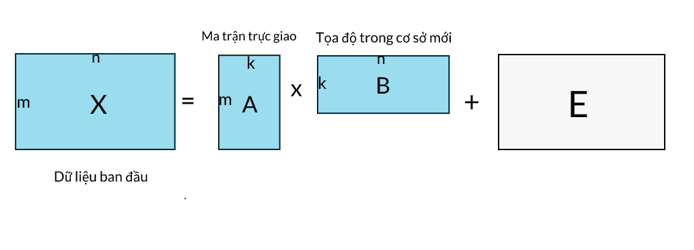
\includegraphics[scale=0.6]{pca_idea.PNG}
	\caption{ Ảnh minh họa PCA}
\end{figure}	
	
\end{frame}

%\begin{frame}{3.3 Mối quan hệ giữa PCA và SVD}
%	
%	
%\end{frame}
\begin{frame}{3.3 Tính duy nhất nghiệm của PCA }
\begin{block}{\textnormal{Định lí}}
Nếu $(\mathbf{A, B})$ là một nghiệm của mô hình PCA thì $(\mathbf{A Q, B Q})$ cũng là một nghiệm của mô hình PCA, với $\mathbf{Q}$ là ma trận trực giao cấp $r$.\\
Lúc này, $\mathbf{Q}$ được gọi là phép quay trực giao.
\end{block}
%
%1) Kiểm tra quan hệ $\sim$ là một quan hệ tương đương trên $\Lp\kgdd$, và mỗi lớp tương đương được xác định bởi
%$$\overline{f}=\lbrace g\in \Lp\kgdd:g\sim f\rbrace.$$
%
%2) Với mọi $ g_1,g_2\in \overline{f}$
%\begin{align*}
%\Vert g_1\Vert_p=\left(\disint_X \vert g_1(x)\vert^p d\mu(x)\right)^{\frac{1}{p}}
%=\left(\disint_{X}\vert g_2(x)\vert^p d\mu(x)\right)^{\frac{1}{p}}
%=\Vert g_2\Vert_p.
%\end{align*}
%Từ đó ta định nghĩa 
%$$\Vert \overline{f}\Vert_p=\Vert g\Vert_p, \text{ với } g\in \overline{f}.$$
\end{frame}

\begin{frame}{3.4 Thuật toán PCA}
\begin{itemize}
	
\item{Bước 1:} Chuẩn hóa dữ liệu.
\item{Bước 2:} Tìm SVD \textquotedblleft chặt cụt\textquotedblright\ của ma trận $\mathbf{X}$, ta được $\mathbf{X}=\mathbf{U}_{r} \mathbf{D}_{r}\left(\mathbf{V}_{r}\right)^{T}$ với $r \leq n$.
\item{Bước 3:} Tìm ma trận $\mathbf{A}$ và $\mathbf{B}$.
\item{Bước 4:} Nếu nghiệm $(\mathbf{A, B})$ chưa tốt thì chọn phép quay $\mathbf{Q}$, với $\mathbf{Q}$ là ma trận trực giao cấp $r$.
\end{itemize}	
\end{frame}


\begin{frame}
	\frametitle{\MakeUppercase{\textsc\bf\large CHƯƠNG 4. Một số ứng dụng của SVD và PCA}}
	\renewcommand{\baselinestretch}{1.5}
	\begin{itemize}
		\item [4.1] \textbf{Ứng dụng của SVD trong xấp xỉ hạng thấp tốt nhất của ma trận}
		\item [4.2] \textbf{Phân tích SVD trong xử lí ảnh}
		%\pause
		%		\item [3.3] \textbf{Mối liên hệ giữa PCA và SVD }
		%\pause
		\item [4.3] \textbf{Ứng dụng của PCA trong nhận dạng khuôn mặt}
		%\pause
		\item [4.4] \textbf{ Nghiên cứu về ứng dụng SVD trong kiến trúc Transformer}
	\end{itemize}
\end{frame}
\begin{frame}{4.1 Ứng dụng của SVD trong xấp xỉ hạng thấp tốt nhất của ma trận}
\begin{block}{\textnormal{{Định lí Eckart- Young, 1936} }}
Với mọi ma trận $\mathbf{B}$ cỡ $m \times n$ và $\operatorname{rank}(\mathbf{B}) \leqslant k$, ta có

$$
\|\mathbf{A}-\mathbf{B}\|_{F} \geqslant\left\|\mathbf{A}-\mathbf{A}_{k}\right\|_{F} .
$$
\end{block}
\end{frame}

\begin{frame}{4.1 Ứng dụng của SVD trong xấp xỉ hạng thấp tốt nhất của ma trận}
	\begin{block}{\textnormal{{Định lí} }}
 Giả sử $\mathbf{A}$ là ma trận cỡ $m \times n$ bất kì, với $\operatorname{rank}(A)=r$ và $\mathbf{A}$ có khai triển kì dị SVD là
$$
\mathbf{A}=\sum_{i=1}^{r} \sigma_{i} \mathbf{u}_{i} \mathcal{V}_{i}^{T} .
$$
Khi đó, với mọi ma trận $\mathbf{B}$ có cỡ $m \times n$ bất kì và $\operatorname{rank}(\mathbf{B}) \leqslant k$, ta có
$$
\|\mathbf{A}-\mathbf{B}\|_{2} \geqslant \sigma_{k+1} .
$$
Dấu \textquotedblleft  =\textquotedblright\ xảy ra khi $\mathbf{B}=\mathbf{A}_{k}=\sum_{i=1}^{k} \sigma_{i} \mathbf{u}_{i} \mathcal{V}_{i}^{T}$.
	\end{block}
\end{frame}

\begin{frame}{4.2 Phân tích SVD trong xử lí ảnh}
	\begin{figure}[htp]
		\centering
		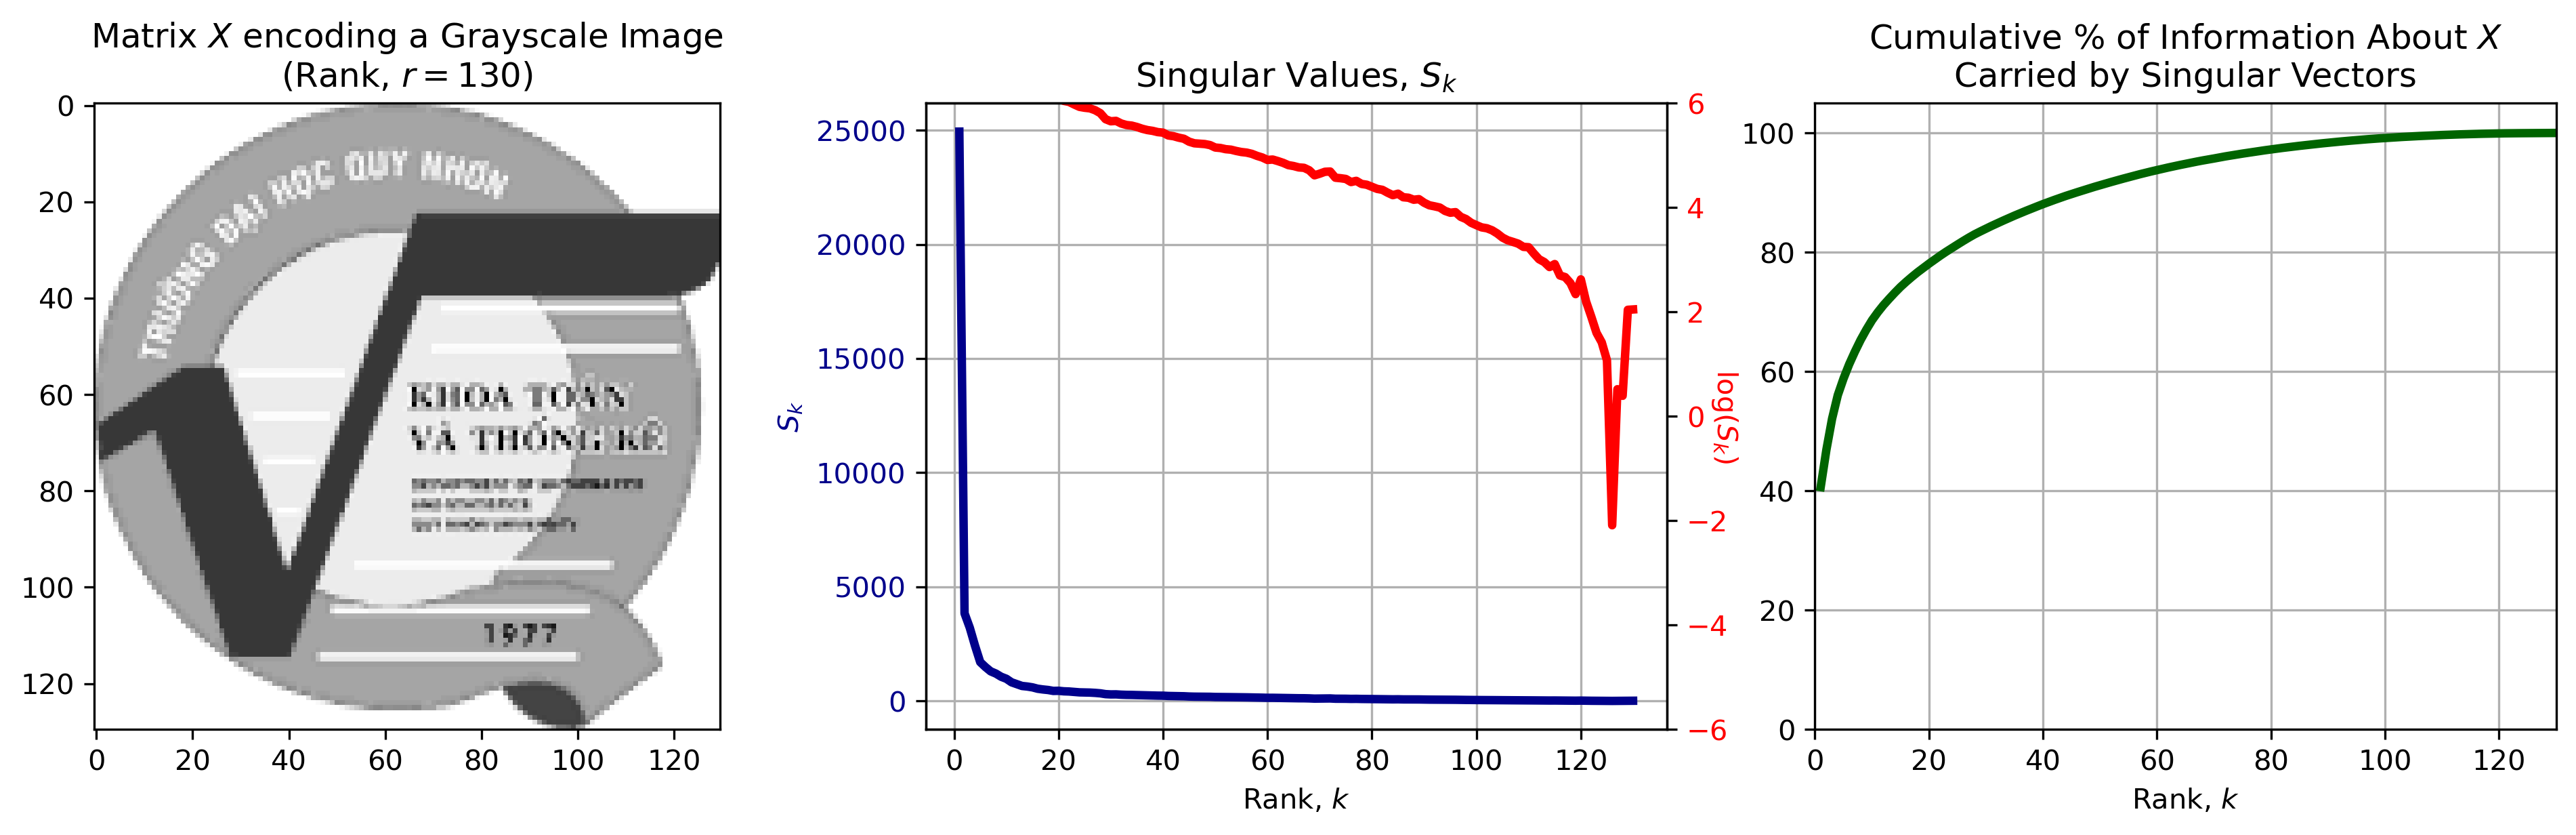
\includegraphics[scale=0.35]{image-singular-values.png}
		\caption{Tính quan trọng của các thành phần chính trong ma trận ảnh và mức độ giữ lại thông tin khi ta giảm số lượng các thành phần chính}
		\label{fig:svd_sigular}
	\end{figure}
\end{frame}

\begin{frame}{4.2 Phân tích SVD trong xử lí ảnh}
\begin{figure}[htp]
	\centering
	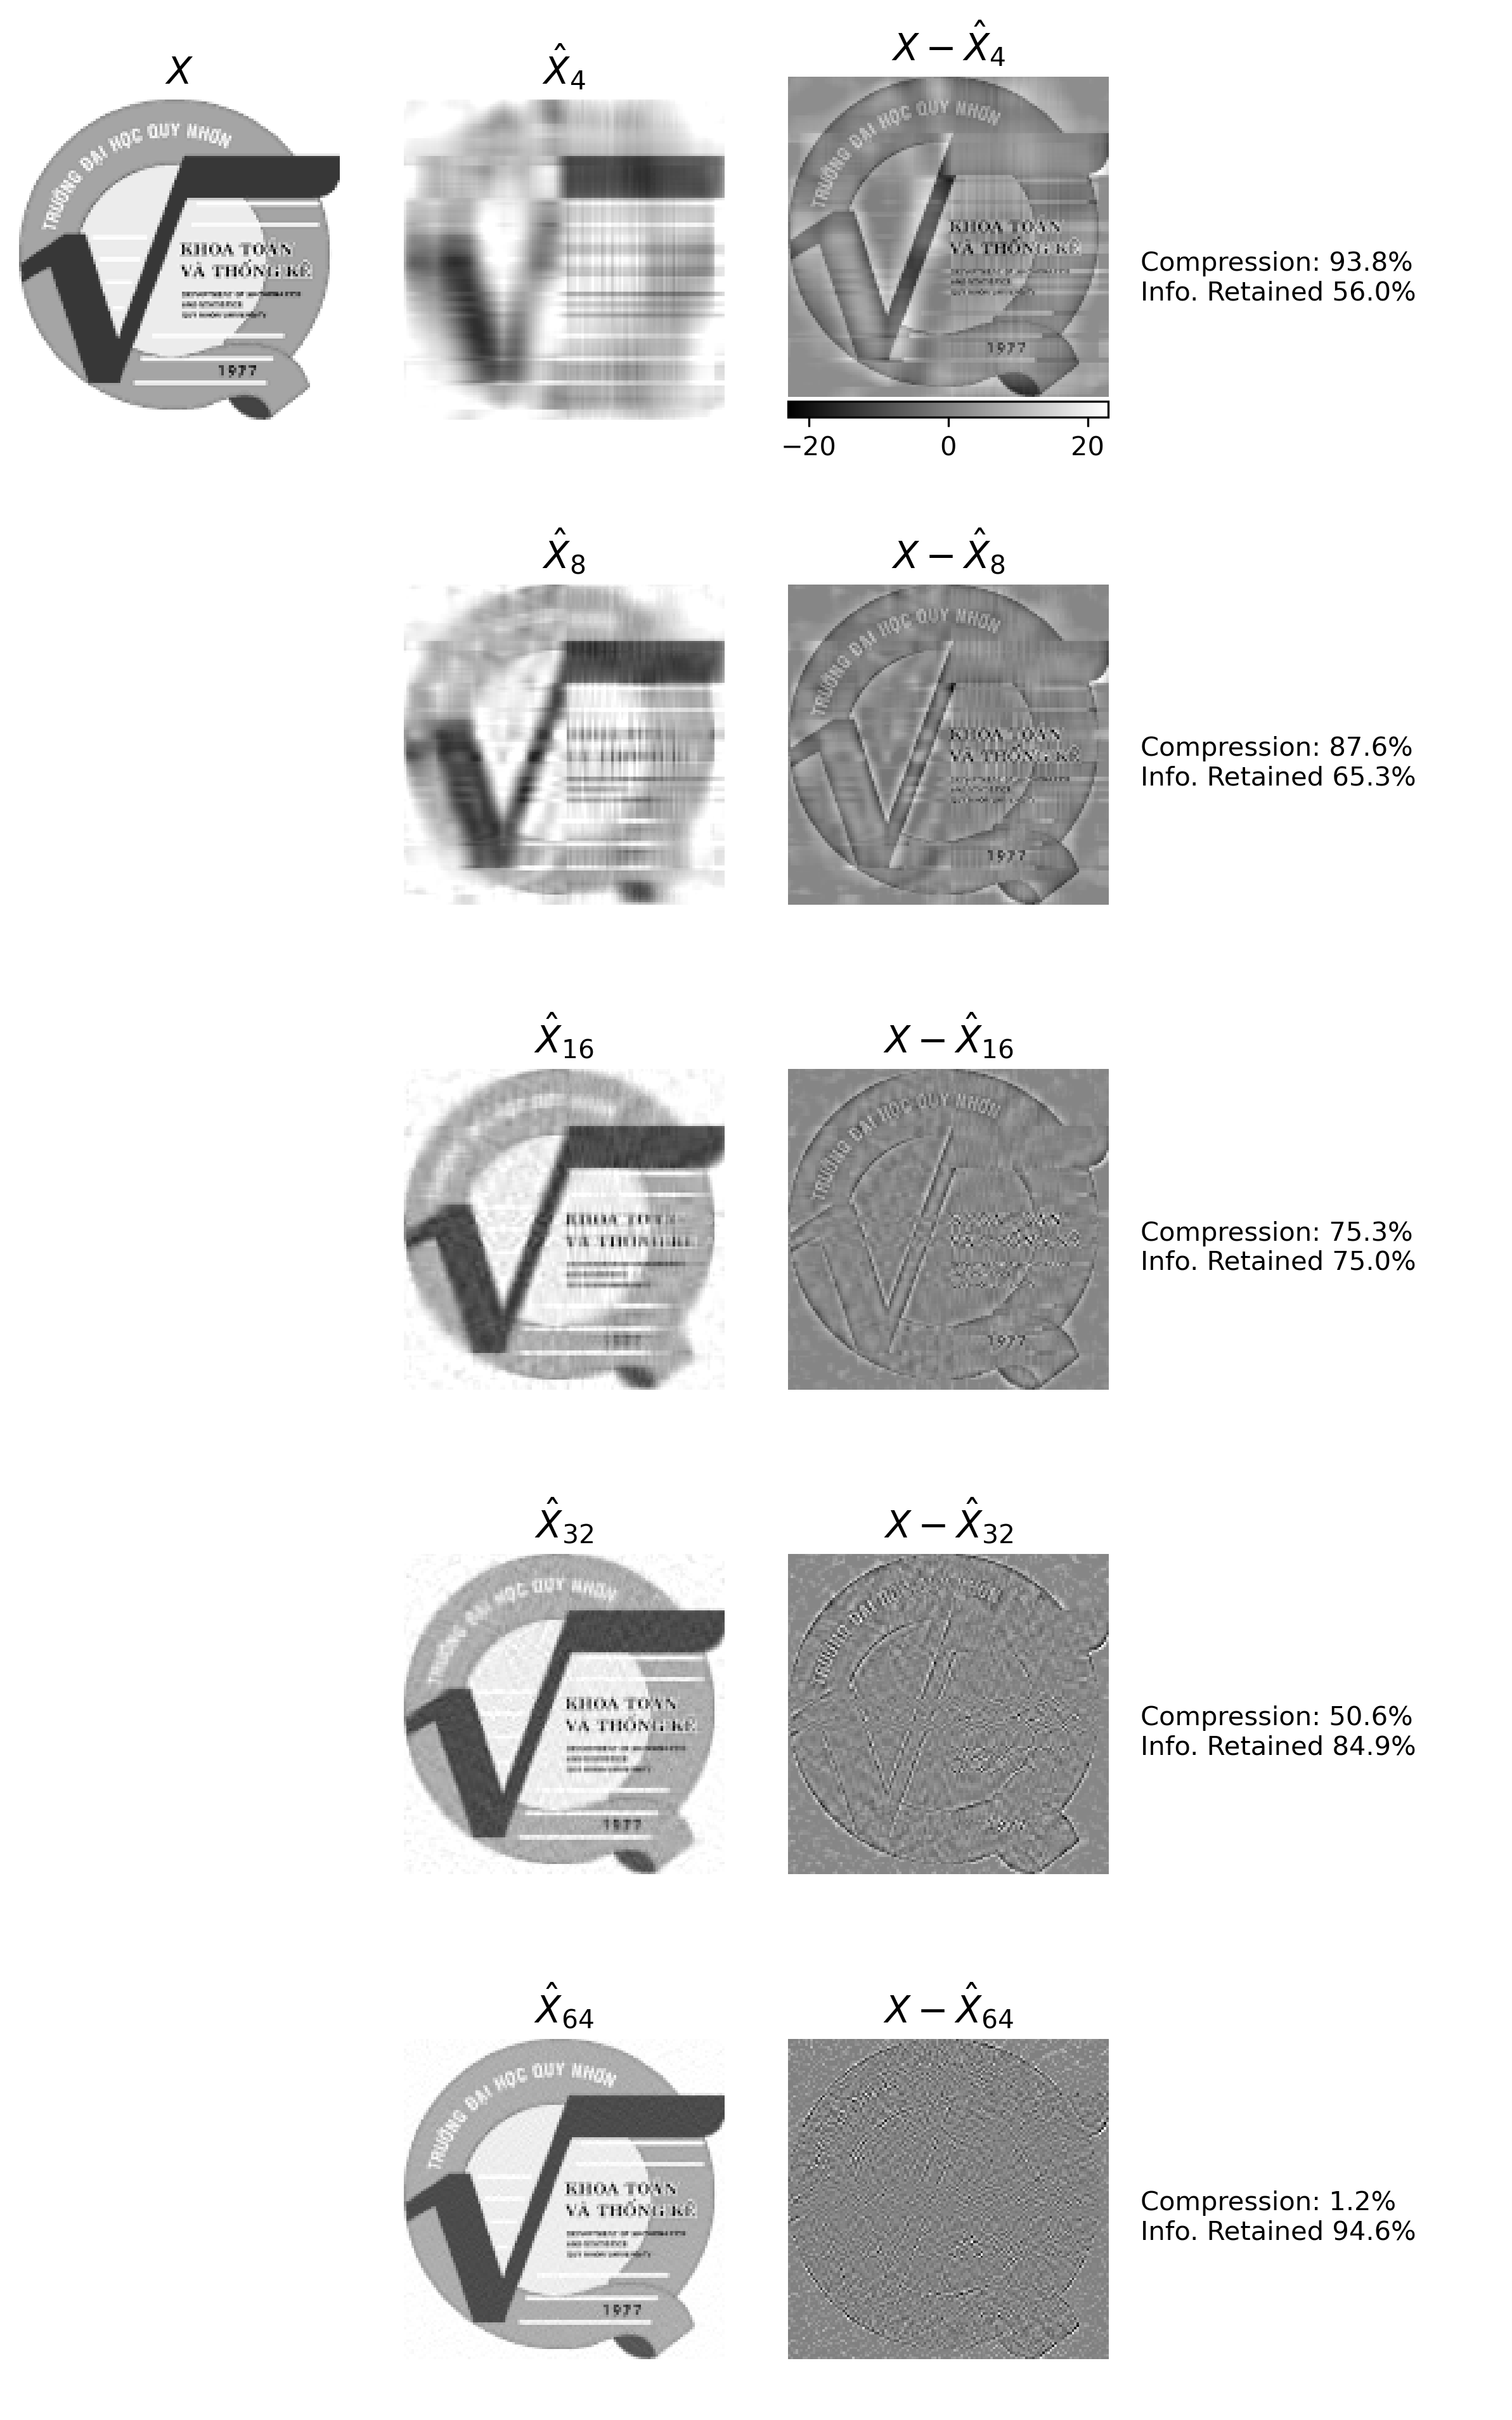
\includegraphics[scale=0.2]{svd_qnu.png}
	\caption{Ứng với từng $k$ ta quan sát được mức độ tối ưu trong việc lưu trữ thông tin cũng như là lượng thông tin được giữ lại.}
	\label{fig:svd_qnu}
\end{figure}
\end{frame}

\begin{frame}{4.3 Ứng dụng của PCA trong nhận dạng khuôn mặt}
	\begin{figure}[htp]
		\centering
		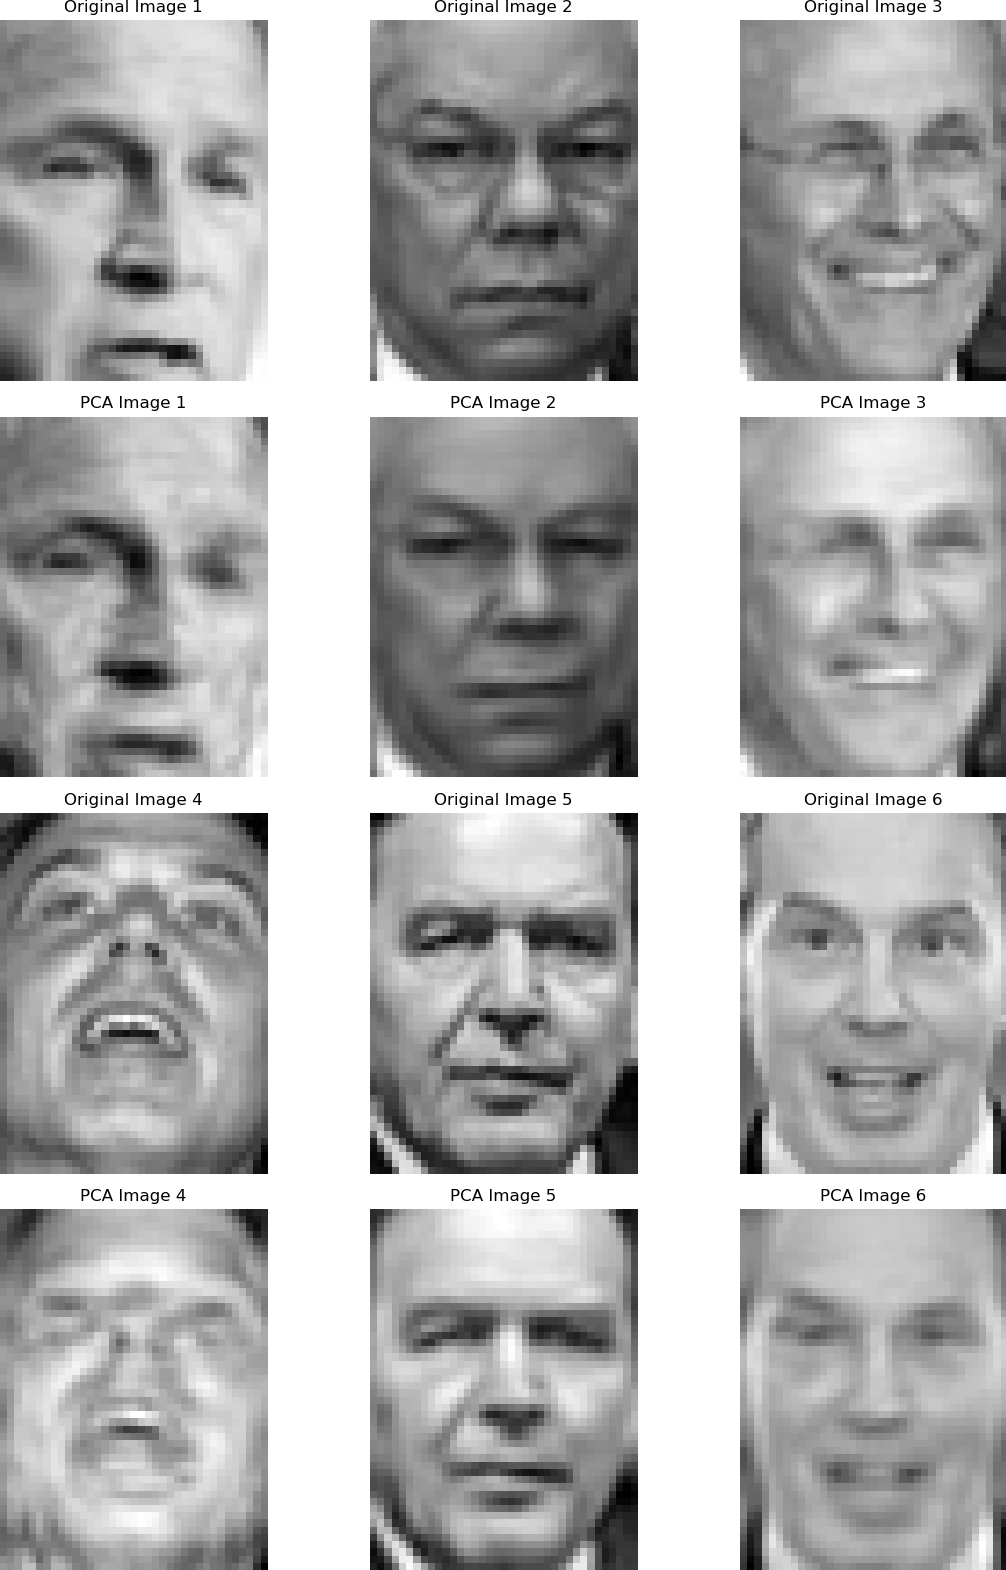
\includegraphics[scale=0.2]{eigenface.png}
		\caption{Hình ảnh ban đầu và hình ảnh sau khi được khôi phục qua PCA.}
		\label{fig:eigenface}
	\end{figure}
\end{frame}

\begin{frame}{4.3 Ứng dụng của PCA trong nhận dạng khuôn mặt}
\begin{figure}[htp]
	\centering
	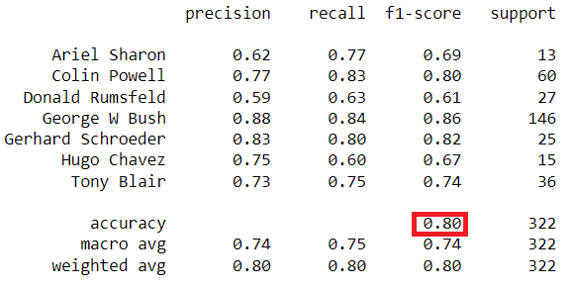
\includegraphics[scale=0.4]{result_svm.png}
	\caption{Báo cáo phân loại sau khi huận luyện bộ phân loại SVM.}
	\label{fig:svm_result}
\end{figure}
\end{frame}

\begin{frame}{4.3 Ứng dụng của PCA trong nhận dạng khuôn mặt}
\begin{figure}[htp]
	\hspace*{-2cm} 
	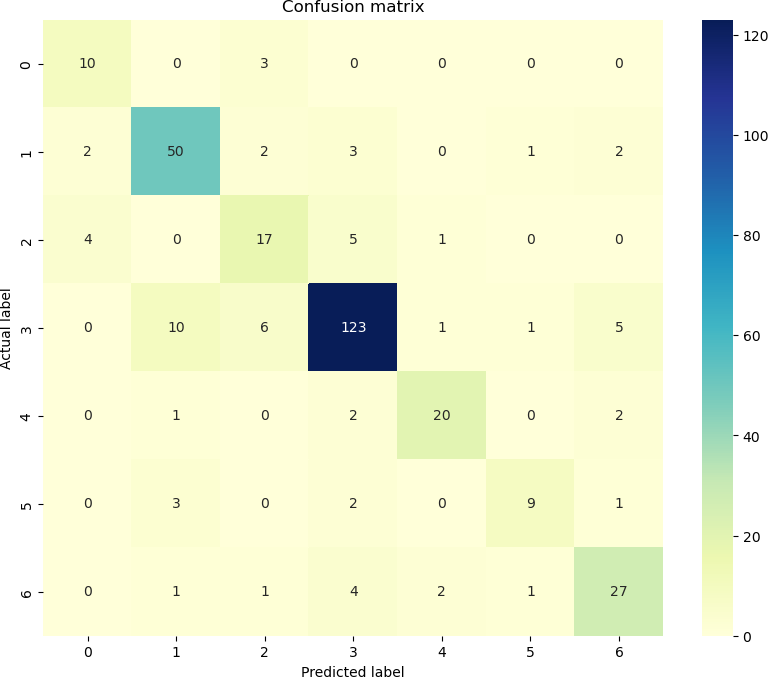
\includegraphics[scale=0.3]{heatmap.png}
	\caption{Ma trận lỗi(confusion matrix)}
	\label{fig:headmap}
\end{figure}
\end{frame}

\begin{frame}{4.3 Ứng dụng của PCA trong nhận dạng khuôn mặt}
\begin{figure}[htp]
	\centering
	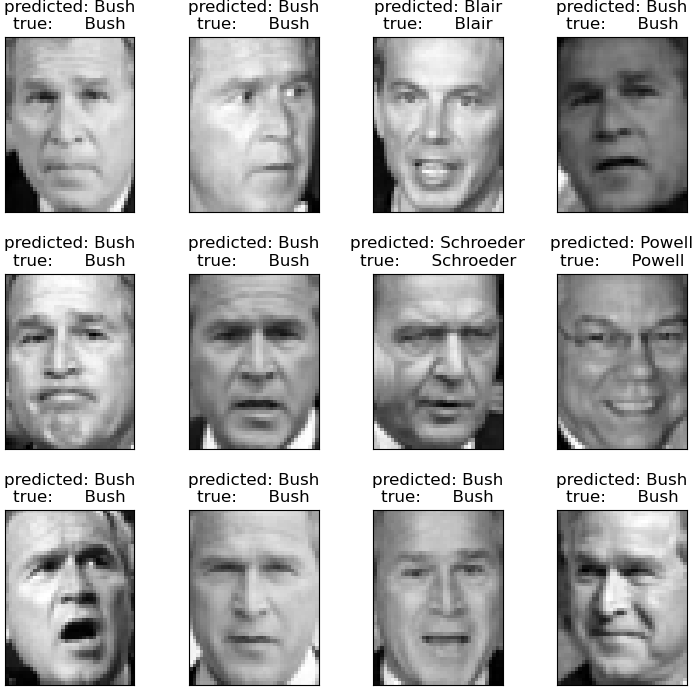
\includegraphics[scale=0.35]{predict_pca.png}
	\caption{kết quả suy luận của bộ phân loại trên tập kiểm thử}
	\label{fig:output}
\end{figure}
\end{frame}


%\begin{frame}{3.2 Không gian $\Lpp\kgdd$ }
%\begin{block}{\textnormal{Định nghĩa 3.2.2}}
%Tập hợp các lớp tương đương $\overline{f}$ của $\Lp\kgdd$ theo quan hệ "$\sim$" được xác định như trên được gọi là \textbf{không gian Lebesgue} $\Lpp\kgdd$,
%$$\Lpp\kgdd=\lbrace \overline{f}:f\in \Lp\kgdd\rbrace.$$
%\end{block}
%Kiểm tra ánh xạ $\Vert \cdot\Vert_{p}: \Lpp\kgdd\to \R^+$ được xác định bởi
%$$\Vert \overline{f}\Vert_p=\Vert f\Vert_p, \quad f\in \overline{f}$$
%thỏa các Tiên đề N1, N2 của chuẩn. Tiên đề N3 có được từ bất đẳng thức Minkowski sau đây:
%\end{frame}
%
%\begin{frame}{3.2 Không gian $\Lpp\kgdd$ }
%\begin{block}{\textnormal{Bất đẳng thức Minkowski.}}
%Cho $1\leq p\leq \infty$ và $f,g\in \Lpp\kgdd$. Khi đó $f+g\in \Lpp\kgdd$ và
%$$\Vert f+g\Vert_p\leq \Vert f\Vert_p+\Vert g\Vert_p.$$
%\end{block}
%\pause
%\begin{block}{\textnormal{Bất đẳng thức Hölder.}}
%Cho $p,q$ là hai số thực không âm thoả $\frac{1}{p}+\frac{1}{q}=1$ và $f\in \Lpp\kgdd$, $g\in\mathit{L}_q\kgdd$. Khi đó $fg\in \mathit{L}_1\kgdd$ và
%\begin{align*}
%\disint_X \vert fg\vert d\mu \leq \Vert f\Vert_p\Vert g\Vert_q.
%\end{align*}
%\end{block}
%\end{frame}
%
%\begin{frame}{3.2 Không gian $\Lpp\kgdd$}
%\begin{block}{\textnormal{Định lý 3.2.8}}
%Cho $1\leq p\leq \infty$. Khi đó, $(\Lpp\kgdd,\Vert \cdot\Vert_p)$ là không gian Banach.
%\end{block}
%Lấy $\lbrace f_n\rbrace_{n\in\N}$ là một dãy Cauchy trong $\Lpp\kgdd$. Ta chỉ ra tồn tại một $f\in\Lpp\kgdd$ và $f_n\rightarrow f$ trong $\Lpp\kgdd$.
%\end{frame}
%\begin{frame}{Chương 3. Phân tích thành phần chính (PCA) }
%Từ bất đẳng thức Chebyshev
%$$\m(\lbrace x\in X:\vert f_n(x)-f_m(x)\vert \geq \epsilon\rbrace)\leq \dfrac{1}{\epsilon^p}\Vert f_n-f_m\Vert_p^p<\epsilon,\quad \forall n,m\geq n_0.$$
%Do đó dãy $ \lbrace f_n\rbrace_n$ là một dãy Cauchy theo độ đo. Vậy tồn tại một dãy con $\lbrace f_{n_k}\rbrace_{k}\subset \lbrace f_n\rbrace_n$ sao cho $ f_{n_k}\to  f$ $\m$-\hkn$ $. Ta chứng minh $f\in\Lpp\kgdd$ và $f_n\rightarrow f$ trong $\Lpp\kgdd$.
%\pause

%$\bullet$ TH2: Lấy $\lbrace f_n\rbrace_{n\in\N}$ là một dãy Cauchy trong $\Loo\kgdd$. 
%$$\vert f_n(x)-f_m(x)\vert\leq \Vert f_n-f_m\Vert_{\infty}<\epsilon,\quad\forall x\in X\setminus E.$$
%Với mỗi $x\in X\setminus E$ thì dãy $\lbrace f_n(x)\rbrace_n$ là dãy Cauchy trong $\R$.
%\begin{subnumcases}{f(x)=}
%\lim_{n\rightarrow\infty} f_n(x) & \text{nếu} $x\in X\setminus E$,\nonumber \\
%0 & \text{nếu} $x\in E$.\nonumber
%\end{subnumcases}
%
%Ta chứng minh $f\in\Loo\kgdd$ và $f_n\to f$ trong $\Loo\kgdd$.
%\end{frame}
%\begin{frame}{3.2 Không gian $\Lpp\kgdd$ }
%\begin{block}{\textnormal{Định lý 3.2.7}}
%Giả sử $f\in\mathit{L}_1\kgdd \cap \mathit{L}_{\infty}\kgdd$. Khi đó
%\begin{itemize}
%\item[(a)] $f\in\Lpp\kgdd$ với $1<p<\infty$.
%\item[(b)] $\lim_{p\rightarrow\infty}\Vert f\Vert_p=\Vert f\Vert_{\infty}.$
%\end{itemize}
%\end{block}
%
%\begin{block}{\textnormal{Định lý 3.2.9}}
%Giả sử $\lbrace f_n\rbrace_{n\in\N}$ là một dãy hàm thuộc $\Lpp\kgdd$, $1\leq p<\infty$, và $f_n\rightarrow f$ $\m$-\hkn, trong đó $f\in\Lpp\kgdd$. Khi đó
%$$f_n\rightarrow f \iff \Vert f_n\Vert_p\rightarrow\Vert f\Vert_p.$$
%\end{block}
%\end{frame}
%
%\begin{frame}{3.3 Các không gian trù mật trong $\Lpp\kgdd$ }
%
%%Giả sử $s=\dissum_{k=1}^n \alpha_k\chi_{E_k} \;,\text{với }\alpha_k\neq 0, 1\leq k\leq n$ và $E_k\in\A$. Nếu $s$ \van thì $\mu(E_k)<\infty, \forall k=\overline{1,n}$, do đó
%%$$ \Vert s\Vert_p^p=\dissum_{k=1}^n \vert \alpha_k\vert^p\mu(E_k)<\infty.$$
%%Suy ra $s \in \Lpp\kgdd$. 
%%\end{frame}
%%
%%\begin{frame}{3.3 Các không gian trù mật trong $\Lpp\kgdd$ }
%%Ngược lại, nếu $s\in \Lpp\kgdd$ thì ta có
%%$$\Vert s\Vert_p^p=\dissum_{k=1}^n \vert \alpha_k\vert^p\mu(E_k)<\infty.$$
%%Nên $\mu(E_k)<\infty, \forall k=\overline{1,n}$. Từ đó ta có
%%$$\mu\left(\lbrace x\in X: s(x)\neq 0\rbrace\right)=\mu(E_1\cup E_2\cup\ldots\cup E_n)=\mu(E_1)+\ldots+\mu(E_n)<\infty.$$
%%Do đó $s$ triệu tiêu bên ngoài một tập có độ đo hữu hạn.
%%\end{frame}
%%
%%\begin{frame}{3.3 Các không gian trù mật trong $\Lpp\kgdd$ }
%\begin{block}{\textnormal{Bổ đề 3.3.1.}}
%Tập tất cả hàm đơn giản mà \van là trù mật trong $\Lpp\kgdd$, với $1\leq p<\infty$.
%\end{block}
%
%$\bullet$ TH 1: $f\geq 0$. Khi đó, tồn tại dãy $\lbrace s_n\rbrace_{n\in \N}$ là dãy hàm đơn giản sao cho  $$0\leq s_n \nearrow f.$$ Ta chỉ ra $s_n \to f$ trong $\Lpp\kgdd$.
%
%$\bullet$ TH 2: $f$ tùy ý. Khi đó $$f=f^+-f^-,$$ với $f^+=\max{\lbrace f,0\rbrace}$ và $f^-=\max{\lbrace -f,0\rbrace}$. Áp dụng TH 1.
%\end{frame}
%
%\begin{frame}{3.3 Các không gian trù mật trong $\Lpp\kgdd$ }
%\begin{block}{\textnormal{Bổ đề 3.3.2.}}
%Tập các hàm đơn giản trù mật trong $\Loo\kgdd$.
%\end{block}
%
%Sử dụng Định lý cấu trúc hàm đo được cho một hàm bị chặn hầu khắp nơi và bởi sự hội tụ trong $\Loo\kgdd$ chính là sự hội tụ đều hầu khắp nơi.
%\end{frame}
%
%%\begin{frame}{3.3 Các không gian trù mật trong $\Lpp\kgdd$ }
%%\begin{block}{\textnormal{Bổ đề 3.3.3.}}
%%Cho $(X,d)$ là một không gian metric, $F$ là một tập đóng trong $X$ và $V$ là một tập mở trong $X$ sao cho $F\subset V$. Khi đó tồn tại một hàm $g:X\rightarrow [0,1]$ sao cho $g$ liên tục trong $X$, $g(x)=1$ với mọi $x\in F$ và $g(x)=0$ với mọi $x\in X\setminus V$.
%%\end{block}
%%\end{frame}
%
%\begin{frame}{3.3 Các không gian trù mật trong $\Lpp\kgdd$ }
%\begin{block}{\textnormal{Định lý 3.3.1.}}
%Cho $f\in \Lpp(\R,\L,m)$ với $1\leq p<\infty$. Khi đó, với mọi $\epsilon>0$, tồn tại một hàm liên tục $g\in \Lpp(\R,\L,m)$ sao cho $\Vert f-g\Vert_p<\epsilon$.
%\end{block}
%
%\begin{block}{\textnormal{Định lý 3.3.2.}}
%Tập hợp tất cả các hàm bước nhảy trù mật trong $\Lpp(\R,\L,m)$ với $1\leq p<\infty$.
%\end{block}
%\end{frame}
%
%%\begin{frame}{3.3 Các không gian trù mật trong $\Lpp\kgdd$ }
%%\begin{block}{\textnormal{Định lý 3.3.2.}}
%%Tập hợp tất cả các hàm bước nhảy trù mật trong $\Lpp(\R,\L,m)$ với $1\leq p<\infty$.
%%\end{block}
%%$\bullet$ TH 1: $f=\chi_{E}$. Chọn $\phi=\chi_{I}$, trong đó $I$ mở sao cho $m(I\setminus E)<\epsilon^p$, thì
%%\begin{align*}
%% \Vert f-\phi\Vert_p<\epsilon.
%%\end{align*}
%%\pause
%%$\bullet$ TH 2: $f=\dissum_{k=1}^n \alpha_k\chi_{E_k}$. Áp dụng Trường hợp 1,
%%$$\Vert \chi_{E_k}-\phi_k\Vert_p<\frac{\epsilon}{n\vert\alpha_k\vert},\quad \forall 1\leq k\leq n.$$
%%Chọn $\phi=\dissum_{k=1}^n \alpha_k\phi_k$, thì
%%$\Vert f-\phi\Vert_p<\epsilon.$
%%\end{frame}
%
%\begin{frame}{3.3 Các không gian trù mật trong $\Lpp\kgdd$ }
%\begin{block}{\textnormal{Định lý 3.3.3.}}
%Không gian $\Lpp(\R,\L,m)$ khả ly với $1\leq p<\infty$.
%\end{block}
% $S=\lbrace \dissum_{k=1}^n b_k \chi_{J_k}:n\in\N,b_k\in\Q\rbrace,$ trong đó $J_k$,$1\leq k\leq n$, là một khoảng hữu hạn với hai đầu mút hữu tỉ.
% % Lấy $\epsilon>0$ và $f\in\Lpp(\R,\L,m)$ ta chứng tỏ tồn tại $b_k\in\Q$ và $J_k$ sao cho
%%\begin{align*}
%%\left\Vert f-\dissum_{k=1}^n b_k\chi_{J_k}\right\Vert_p\leq \epsilon.
%%\end{align*}
%\end{frame}
%
%\begin{frame}{3.4 Các không gian đối ngẫu }
%\begin{block}{\textnormal{Bổ đề 3.4.1.}}
%Cho $\kgdd$ là một không gian độ đo hữu hạn. Giả sử $g\in \mathit{L}_1\kgdd$ sao cho với bất kỳ $M>0$ và mọi hàm đơn giản $s\in\Lpp\kgdd$ xảy ra $$\left\vert \disint_X sg\,dm\right\vert\leq M\Vert s\Vert_p$$
%với $1\leq p<\infty$. Khi đó $g\in \mathit{L}_q\kgdd$ và $\Vert g\Vert_q\leq M$.
%\end{block}
%\end{frame}
%
%\begin{frame}{3.4 Các không gian đối ngẫu }
%\begin{block}{\textnormal{Định lý Riesz}}
%Cho $\kgdd$ là một không gian độ đo $\sigma$-hữu hạn\\
%$\bullet$ Với mỗi $g\in\mathit{L}_q\kgdd$ thì xác định một phiếm hàm tuyến tính liên tục $F$ trên $\Lpp\kgdd$ được cho bởi
%$$F(f)=\disint_X fg\,d\m,$$
%và $\Vert F\Vert=\Vert g\Vert_q.$\\
%$\bullet$ Với mỗi $F$ là một phiếm hàm tuyến tính liên tục trên $\Lpp\kgdd$. Khi đó tồn tại duy nhất hàm $g\in\mathit{L}_q\kgdd$ sao cho 
%$$F(f)=\disint_X fg\,d\m,\quad f\in\Lpp\kgdd.$$
%Hơn nữa $\Vert F\Vert=\Vert g\Vert_q$.
%\end{block}
%\end{frame}
%
%%\begin{frame}{3.4 Các không gian đối ngẫu }
%%\begin{block}{\textnormal{Định nghĩa 3.4.1.}}
%%Cho $\kgdd$ là một không gian độ đo và $\nu: \A \to \R$ là một hàm cộng tính trên $\sigma$-đại số $\A$. Ta định nghĩa hàm \textbf{biến phân toàn phần} $\vert \nu\vert: \A \to [0,\infty]$ như sau
%%$$\vert \nu \vert(A)=\sup \left\lbrace \dissum_{i=1}^n \vert \nu(A_i)\vert: (A_i)_{i=1}^n\subset\A \text{ và }A=\sqcup_{i=1}^n A_i\right\rbrace$$
%%với mọi $A\in \A$. Hàm $\nu$ được gọi là \textbf{độ đo có dấu cộng tính bị chặn} nếu $\vert \nu\vert(X)<\infty$. Trong trường hợp này, ta ký hiệu
%%$$\Vert \nu\Vert_{\text{var}}:=\vert \nu\vert(X).$$
%%\end{block}
%%\end{frame}
%
%\begin{frame}{3.4 Các không gian đối ngẫu }
%Ký hiệu $\mathfrak{BA}\kgdd$ là tập hợp tất cả các độ đo có dấu cộng tính bị chặn và liên tục tuyệt đối với độ đo dương $\mu$. Trên đó ta định nghĩa
%%\begin{block}{\textnormal{Mệnh đề 3.4.1.}}
%%Cho $(X,\A)$ là một không gian đo được và $\nu:\A\to \R$ là một hàm cộng tính. Khi đó 
%%\begin{itemize}
%%\item[a)] $\vert \nu\vert \geq 0$ và $\vert\nu\vert(\emptyset)=0.$
%%\item[b)] $\vert \nu\vert $ cộng tính trên $\A$.
%%\item[c)] $\vert \nu\vert $ cộng tính hữu hạn trên $\A$.
%%\item[d)] $\vert \nu\vert $ đơn điệu trên $\A$.
%%\item[e)] $\vert \nu(A)\vert \leq \vert \nu\vert(A)$ với mọi $A\in\A$.
%%\item[g)] Nếu $\nu \geq 0$ thì $\vert \nu\vert =\nu$.
%%\end{itemize}
%%\end{block}
%$$\Vert \nu\Vert_{\text{var}}:=\vert \nu\vert(X)=\sup \left\lbrace \dissum_{i=1}^n \vert \nu(A_i)\vert: (A_i)_{i=1}^n\subset\A \text{ và }X=\sqcup_{i=1}^n A_i\right\rbrace.$$
%
%\begin{block}{\textnormal{Mệnh đề 3.4.2.}}
%Cho $\kgdd$ là một không gian độ đo. Khi đó $\Vert \cdot\Vert_{\text{var}}$ là một chuẩn trên $\mathfrak{BA}\kgdd$.
%\end{block}
%\end{frame}
%
%\begin{frame}{3.4 Các không gian đối ngẫu }
%\begin{block}{\textnormal{Định nghĩa 3.4.2.}}
%Cho $(X,\A)$ là một không gian đo được và $\nu: \A \to \R$ là một độ đo có dấu cộng tính bị chặn. Với mọi $f$ là một hàm đơn giản trên $A$, ta định nghĩa tích phân của $f$ trên $A$ ứng với $\nu$ là
%$$\disint_A f(x)d\nu(x):=\dissum_{i=1}^n \alpha_i\nu(A_i),$$
%ở đây $f=\dissum_{i=1}^n \alpha_i\chi_{A_i}$ là biển diễn chính tắc của $f$ trên $A$.
%\end{block}
%\end{frame}
%
%%\begin{frame}{3.4 Các không gian đối ngẫu }
%%\begin{block}{\textnormal{Định lý 3.4.3.}}
%%Toán tử tích phân trong Định nghĩa 3.4.2 là toán tử tuyến tính.
%%\end{block}
%%\begin{block}{\textnormal{Mệnh đề 3.4.3.}}
%%Cho $(X,\A)$ là một không gian đo được và $\nu: \A \to \R$ là một độ đo có dấu cộng tính bị chặn và $f$ là một hàm đơn giản. Khi đó
%%$$\left\vert \disint_X f(x)d\nu(x)\right\vert\leq \Vert \nu\Vert_{\text{var}}\sup_{x\in X}\vert f(x)\vert.$$
%%\end{block}
%%\end{frame}
%
%\begin{frame}{3.4 Các không gian đối ngẫu }
%\begin{block}{\textnormal{Định nghĩa 3.4.3.}}
%Cho $(X,\A)$ là một không gian đo được, $\nu:\A\to \R$ là một độ đo có dấu cộng tính bị chặn và $f:X\to \R$ là một hàm đo được và bị chặn trên $X$. Ta định nghĩa tích phân của $f$ trên $X$ ứng với $\nu$ cho bởi
%$$\disint_X f(x)d\nu(x)=\lim_{n\to\infty} \disint_X f_n(x)d\nu(x),$$
%trong đó $\lbrace f_n\rbrace_{n=1}^{\infty}$ là một dãy hàm đơn giản và hội tụ đều đến $f$ trên $X$.
%\end{block}
%\end{frame}
%
%\begin{frame}{3.4 Các không gian đối ngẫu }
%\begin{block}{\textnormal{Bổ đề 3.4.3.}}
%Cho $(X,\A)$ là một không gian đo được, $\nu:\A\to \R$ là một độ đo có dấu cộng tính bị chặn. Giả sử $f:X\to \R$ là một hàm đo được và bị chặn trên $X$. Khi đó\\
%a) Với mọi dãy hàm đơn giản $\lbrace f_n\rbrace_{n=1}^{\infty}$ thoả mãn $f_n(x)\rightrightarrows f(x)$ trên $X$ thì tồn tại giới hạn
%$$\lim_{n\to\infty}\disint_X f_n(x)d\nu(x).$$
%b) Nếu $\lbrace f_n\rbrace_{n=1}^{\infty}$ và $\lbrace g_n\rbrace_{n=1}^{\infty}$ là hai dãy hàm đơn giản thoả mãn $f_n(x)\rightrightarrows f(x)$ và $g_n(x)\rightrightarrows f(x)$ trên $X$ thì
%$$\lim_{n\to\infty}\disint_X f_n(x)d\nu(x)=\lim_{n\to\infty}\disint_X g_n(x)d\nu(x).$$
%\end{block}
%\end{frame}
%
%\begin{frame}{3.4 Các không gian đối ngẫu }
%\begin{block}{\textnormal{Định nghĩa 3.4.4.}}
%Cho $\kgdd$ là một không gian độ đo và $\nu\in\mathfrak{BA}\kgdd$. Với mọi $f\in\Loo\kgdd$ ta định nghĩa tích phân của $f$ trên $X$ ứng với $\nu$ cho bởi
%$$\disint_X f(x)d\nu(x)=\lim_{n\to\infty} \disint_X f_n(x)d\nu(x),$$
%với $\lbrace f_n\rbrace_{n=1}^{\infty}$ là một dãy hàm đơn giản và hội tụ đều đến $f$ trên $X\setminus Y$ trong đó $Y$ là một tập có độ đo không.
%\end{block}
%
%\begin{block}{\textnormal{Mệnh đề 3.4.4.}}
%Nếu $f=g\; \m$-\hkn, thì 
%$$\disint_X f(x)d\nu(x)=\disint_X g(x)d\nu(x).$$
%\end{block}
%\end{frame}
%
%\begin{frame}{3.4 Các không gian đối ngẫu }
%\begin{block}{\textnormal{Mệnh đề 3.4.5.}}
%Toán tử tích phân trong Định nghĩa 3.4.4 là toán tử tuyến tính.
%\end{block}
%\begin{block}{\textnormal{Mệnh đề 3.4.6.}}
%Cho $\kgdd$ là một không gian độ đo và $\nu\in\mathfrak{BA}\kgdd$. Khi đó
%$$\left\vert \disint_X f(x)d\nu(x) \right\vert\leq \Vert \nu\Vert_{\text{var}}\Vert f\Vert_{\infty}$$
%với mọi $f\in\Loo\kgdd.$
%\end{block}
%\end{frame}
%
%\begin{frame}{3.4 Các không gian đối ngẫu }
%\begin{block}{\textnormal{Định lý biểu diễn Kantorovich.}}
%Cho $\kgdd$ là một không gian độ đo. Khi đó\\
%a) Với mỗi $\nu\in\mathfrak{BA}\kgdd$, thì phiếm hàm $F:\Loo\kgdd\to \R$ xác định bởi
%$$F(f)=\disint_X f(x)d\nu(x),\qquad\forall f\in \Loo\kgdd$$
%là một phiếm hàm tuyến tính liên tục trên $\Loo\kgdd$.\\
%b) Với mỗi $F$ là phiếm hàm tuyến tính liên tục trên $\Loo\kgdd$ tồn tại duy nhất phần tử $\nu\in\mathfrak{BA}\kgdd$ sao cho
%$$F(f)=\disint_X f(x)d\nu(x),\qquad\forall f\in \Loo\kgdd.$$
%Hơn nữa $\Vert \nu\Vert_{\text{var}}=\Vert F\Vert.$ 
%\end{block}
%\end{frame}
%
%\begin{frame}{3.5 Sự hội tụ yếu }
%%\begin{block}{\textnormal{Định nghĩa 3.5.1.}}
%%Cho $\kgdd$ là một không gian độ đo, $1\leq p<\infty$ và $q$ là số mũ liên hợp của $p$. Một dãy hàm $\lbrace f_n\rbrace_{n\in\N}$ thuộc $\Lpp\kgdd$, $1\leq p<\infty$ được gọi là \textbf{hội tụ yếu} đến hàm $f\in\Lpp\kgdd$ nếu
%%$$\lim_{n\rightarrow\infty} \disint_X f_ng\,\text{d}\m=\disint_X fg\,\text{d}\m$$
%%với mọi $g\in\mathit{L}_q\kgdd$, và được ký hiệu là $f_n\rightharpoonup f$.
%%\end{block}
%
%\begin{block}{\textnormal{Định lý 3.5.1.}}
%Cho $\kgdd$ là một không gian độ đo hữu hạn và $1<p<\infty$. Đặt $\lbrace f_n\rbrace_{n\in\N}$ là một dãy hàm trong $\Lpp\kgdd$ sao cho $f_n\rightarrow f$ $\m$-\hkn. Khi đó $f_n\rightharpoonup f$ khi và chỉ khi $\lbrace\Vert f_n\Vert_p\rbrace_{n\in\N}$ bị chặn.
%\end{block}
%\pause
%\begin{block}{\textnormal{Định lý 3.5.2.}}
%Giả sử $\lbrace f_n\rbrace_{n\in\N}\subset\Lpp(\R)$ với $M=\sup_n\Vert f_n\Vert_p<\infty$. Khi đó tồn tại $f\in\Lpp(\R)$ sao cho $\Vert f\Vert_p\leq M$ và một dãy con $\lbrace f_{n_k}\rbrace_{k\in\N}\subset \lbrace f_n\rbrace_{n\in\N}$ sao cho $$f_{n_k}\rightharpoonup f.$$
%\end{block}
%\end{frame}

\begin{frame}{Tài liệu tham khảo}
\begin{thebibliography}{99}
	\bibitem{1} L. Đ. Kỳ, \textit{Bài giảng về Lý thuyết độ đo và tích phân}, Quy Nhơn, 2018.
	\bibitem{2} L. Đ. Kỳ, \textit{Bài giảng về Giải tích thực}, Quy Nhơn, 2018.
	\bibitem{3} T.T. Quang, \textit{Cơ sở lý thuyết Giải tích hàm}, Quy nhơn, 2013.
	\bibitem{4} H. Brezis, \textit{Functional analysis}, Sobolev spaces and partial differential equations. Universitext. Springer, New York, 2011.
	\bibitem{5} R. E. Castillo and H. Rafeiro, \textit{An introductory course in Lebesgue spaces}, CMS Books in Mathematics/Ouvrages de Mathématiques de la SMC. Springer, [Cham], 2016.
	\bibitem{6} H. L. Royden, \textit{Real analysis}. Fourth edition. Pearson Education and China Machine Press, China, 2010.
\end{thebibliography}
\end{frame}
\begin{frame}
\centerline{\Large\bf \fontsize{18}{18}\selectfont{\color{red}{KẾT THÚC BÁO CÁO}}}
\vspace{1cm}
\centerline{\Large\bf \fontsize{23}{18}\selectfont{\color{blue}{TRÂN TRỌNG CẢM ƠN!}}}

\end{frame}
\end{document} 
